\documentclass[10pt,a4paper]{amsart}
\usepackage[margin=19mm]{geometry}
\usepackage{amsmath,amssymb,mathtools}
\usepackage[scr=rsfs,cal=euler]{mathalfa}
\usepackage{xfrac}
\usepackage[unicode,hidelinks,bookmarks=false]{hyperref}
\newcommand{\ie}{i.e.\ }
\newcommand{\cf}{cf.\ }
\newcommand{\resp}{respectively\ }
\newcommand{\Subsection}{\subsection}
\providecommand{\nobreakdash}{\nobreak\hbox{-}}
\setlength{\emergencystretch}{2em}
\multlinegap0pt
\usepackage{tikz}
\usepackage{amssymb}
\newtheorem{lemma}{Lemma}
\newtheorem{corollary}{Corollary}
\renewcommand\ge{\geqslant}\renewcommand\le{\leqslant}
\title{Information Inequalities for Five Random Variables}
\author{E.P. Csirmaz, L. Csirmaz}
\date{Source: arXiv:2512.23316v2 (CC BY 4.0)}
\begin{document}
\maketitle

\noindent\emph{Source and licence.} Information Inequalities for Five Random Variables. Version arXiv:2512.23316v2 (CC BY 4.0), distributed by arXiv under the Creative Commons Attribution 4.0 International licence, http://creativecommons.org/licenses/by/4.0/, as recorded in the arXiv licence metadata for this exact version and shown on the abstract page https://arxiv.org/abs/2512.23316v2. Full licence notice: \texttt{licenses/arxiv-2512.23316-CC-BY-4.0.txt}.\par\smallskip

\noindent\textit{Editorial scope.} Counted unit: the article's corollary corr1 (source0.tex lines 2034--2039). The article's complete original proof of it is delivered with it (source0.tex lines 2041--2115, one \texttt{proof} environment of 75 lines). No mathematics is written, repaired or re-derived: the statement and the proof are the article's own lines, in the article's own notation, and no retained line is substituted or re-flowed.  Retained uncounted as the source-local context the proof needs: lines 1884--1900.  Nothing was omitted from any retained span, so the package carries no omission record.  No retained line contains a citation, so the wrapper carries no bibliography and no bibliography entry.  The retained lines contain the article's own diagram code, which the wrapper typesets with the standard tikz packages; no image file is delivered and the package declares no asset dependency.  Editorial formatting only, in addition: an AMS \texttt{amsart} preamble that restates the article's own declarations and macros used by the retained lines, namely the environments \texttt{lemma}, \texttt{corollary} on separate counters, together with the standard packages those lines need.  The retained environments print in this document as Lemma 1, Corollary 1 in order of appearance, whereas the article prints the same items with the numbering of its own full document.  The complete native source of the article as distributed in the arXiv e-print for this exact version is bundled unchanged as \texttt{sources/191796/source0.tex}.
\begin{lemma}\label{lemma:convex}
Let $i_1<i_2<i_3$, and $j_1>j_2>j_3$.
\begin{itemize}
\item[(i)] $\mathbf v_S$ is
superseded by the vectors $\{\mathbf v_{S+(i_1,j_1)},
\mathbf v_{S-(i_2,j_2)}, \mathbf v_{S+(i_3,j_3)} \}$ if and only if
$$
    \frac{~j_2-j_3~}{i_3-i_2} \ge \frac{~j_1-j_3~}{i_3-i_1}.
$$
\item[(ii)] $\mathbf v_S$ is superseded by
$\{\mathbf v_{S-(i_1,j_1)}, \mathbf v_{S+(i_2,j_2)}, \mathbf
v_{S-(i_3,j_3)} \}$ if and only if
$$
    \frac{~j_2-j_3~}{i_3-i_2} \le \frac{~j_1-j_3~}{i_3-i_1}.
$$
\end{itemize}
\end{lemma}

\begin{corollary}\label{corr1}
If for some $S\subseteq D_n$ the vector $\mathbf v_S$ is not superseded by
other vectors generated from subsets of $D_n$, then either the sequence
$S^{\mathrm {col}}$ is strictly decreasing, or the sequence
$S^{\mathrm{row}}$ is strictly decreasing.
\end{corollary}

\begin{proof}
If $S^{\mathrm{col}}$ is not strictly decreasing, then the upper bound of
$S$ contains a horizontal segment of length at least $2$. Similarly, if
$S^{\mathrm{row}}$ is not strictly decreasing, then the right bound of $S$
contains a vertical segment of length at least $2$, see Figure
\ref{fig:corr1}. Take such a horizontal and a vertical segments whose
distance is minimal. Let the horizontal segment be in row $r$ between
columns $c_1$ and $c_2$, and the vertical segment be in column $c$ between
rows $r_1$ and $r_2$. The horizontal and vertical segments are connected by
(a possibly empty) diagonal staircase. Depending on which segment comes
first, there are two possible arrangements as depicted on Figure
\ref{fig:corr1}.
%%%%%%%%%%%%%%%%%%%%%%%%%%%%%%%%%%%%%%%%%%
\begin{figure}[h!tb]
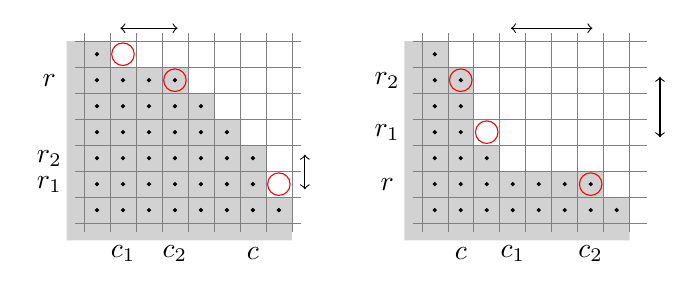
\begin{tikzpicture}[scale=1.1]
\def\dd(#1,#2){\filldraw[black] (\x+0.3*#1,\y+0.3*#2) circle (0.5pt);}
\def\cc(#1,#2){\draw[red] (\x+0.3*#1,\y+0.3*#2) circle (0.13cm);}
\def\ss#1{#1}
\draw[<->] (0.42,2.25) -- (0.18+0.9,2.25);
\draw[<->] (2.55,0.15+0.64) -- (2.55,0.15+0.24);
\fill[gray!35] (-0.2,-0.2)--(-0.2,2.1)--(0.3,2.1)--(0.3,1.8)--(1.2,1.8)
      --(1.2,1.5)--(1.5,1.5)--(1.5,1.2)--(1.8,1.2)--(1.8,0.9)--(2.1,0.9)
      --(2.1,0.3)
      --(2.4,0.3)--(2.4,-0.2)--cycle;
\draw (-0.4,1.65) node {$\ss r$};
\draw (-0.4,0.45) node {$\ss r_1$};
\draw (-0.4,0.75) node {$\ss r_2$};
\draw (0.45,-0.35) node{$\ss c_1$};
\draw (1.05,-0.35) node{$\ss c_2$};
\draw (1.95,-0.35) node{$\ss c$};
\draw[step=0.3cm,help lines] (-0.1,-0.1) grid (2.5,2.2);
\def\x{0.15}\def\y{0.15}
\foreach\j/\k in {0/6,1/5,2/5,3/5,4/4,5/3}{
\foreach\i in {0,...,\k}{\dd(\j,\i)}}
\foreach\i in {0,1,2}{\dd(6,\i)} \dd(7,0)
           \cc(1,6)\cc(3,5)\cc(7,1)
\draw[<->] (4.03+0.9,2.25)--(4.07+1.8,2.25);
\draw[<->] (6.65,0.15+1.54)--(6.65,0.15+0.84);
\fill[gray!35] (3.7,-0.2)--(3.7,2.1)--(4.2,2.1)--(4.2,1.8)--(4.5,1.8)--(4.5,0.9)
      --(4.8,0.9)--(4.8,0.6)--(6.0,0.6)--(6.0,0.3)--(6.3,0.3)--(6.3,-0.2)
      --cycle;
\draw[step=0.3cm,help lines] (3.8,-0.1) grid (6.5,2.2);
\def\x{4.05}
\foreach\i in{0,...,6}{\dd(0,\i)}
\foreach\i in{0,...,5}{\dd(1,\i)}
\foreach\i in{0,1,2}{\dd(2,\i)}
\foreach\i in{0,1}{\dd(3,\i)\dd(4,\i)\dd(5,\i)\dd(6,\i)} \dd(7,0)
     \cc(1,5)\cc(2,3)\cc(6,1)
\draw (3.5,0.45) node{$\ss r$};
\draw (3.5,1.05) node{$\ss r_1$};
\draw (3.5,1.65) node{$\ss r_2$};
\draw (4.35,-0.35) node{$\ss c$};
\draw (4.95,-0.35) node{$\ss c_1$};
\draw (5.85,-0.35) node{$\ss c_2$};
\end{tikzpicture}
\caption{Nearest horizontal and vertical boundary segments of the gray
region are marked by the arrows. Red circles indicate points to be added and
subtracted.
}\label{fig:corr1}
\end{figure}
%%%%%%%%%%%%%%%%%%%%%%%%%%%%%%%%%%%%%%%%%%%%%%%%%%%%%%%%%%%%
In the first case $c_1<c_2<c$, and $r_1<r_2<r$; in the second case
$c<c_1<c_2$ and $r<r_1<r_2$. Apply Lemma \ref{lemma:convex} to the marked
points and observe that the modified downward closed sets are always subsets
of $D_n$. In the first case
$$
   \frac{c_2-c_1}{(r+1)-r} \ge 1 \ge \frac{c+1-c_2}{r_1-r},
$$
and in the second case
$$
   \frac{(c+1)-c)}{r_1-r_2} \le 1 \le \frac{c_2-(c+1)}{r-r_1}.
$$
Therefore, by Lemma \ref{lemma:convex}, $\mathbf v_S$ is superseded by the
vectors generated by the indicated sets, proving the claim.
\end{proof}

\end{document}
